\documentclass[11pt,a4paper,DIV=9]{scrartcl}

\usepackage{tikz}
\usepackage{ngerman}
\usepackage[utf8]{inputenc}
\usepackage{amsmath,amssymb}
\usepackage{hyperref}
\hypersetup{linktoc=all}
% Schriftart ändern
\renewcommand{\rmdefault}{ppl}
%Möglichkeit zur Änderung von Überschriften
\usepackage{sectsty}
%Überschrift \section uandern
\definecolor{blue}{RGB}{76 , 92, 153}
\allsectionsfont{\color{blue}}
\paragraphfont{\color{blue}}

%Variable Blattnummer
\newcommand{\blatt}[1]{
  \newcommand{\blattnr}{#1}
}
%Aufgabe und Aufgabenteil definieren
\newcounter{temp}
\newcommand{\aufgabe}[1]{
  \setcounter{temp}{\value{subsection}}
  \setcounter{subsection}{#1}
  \addtocounter{subsection}{-1}
  \subsection{Aufgabe}
  \setcounter{subsection}{\value{temp}}
}
\newcommand{\teil}[2][]{
  \subsubsection*{#2) #1}
}
\renewcommand{\author}[1]{\renewcommand{\author}{#1}}
\renewcommand{\title}[1]{\renewcommand{\title}{#1}}
\newcommand{\makehomeworktitle}{
  \begin{minipage}[t]{6.5cm}
    \sf{\author}
  \end{minipage}
  \begin{minipage}[t]{6.5cm}
    \begin{flushright}
      \sf{\title\\\today}
    \end{flushright}
  \end{minipage}
  \\[0.2cm]
  \begin{center}
    \sf{
      \color{blue}{
        \LARGE{Dokumentation First.FM}
      }
    }
  \end{center}
  \vspace{0.1cm}
}

%%%%%%%%%%%%%%%%%%%%%%%%
%%% Statisch
\author{{[}4131658{]} Jan Germann \\{[}4054962{]} Christian Ratz\\Übungsgruppe 1}
\title{SQL Praktikum}

%%% Auf jedes Hausaufgabenblatt anpassen
\blatt{1}
%%%%%%%%%%%%%%%%%%%%%%%%
\begin{document}
\makehomeworktitle
\tableofcontents
\newpage
\section{Einleitung}
  \subsection{Allgemeines}
    // TODO Einleitung anpassen.

  \subsection{Formatierung} 
    In der Dokumentation sowie im dazugehörigen Diagramm gilt die folgende Formatierung.

    \begin{description}
      \item [Klassennamen] \hfill \\
        Der Name einer Klasse ist im Regelfall \textbf{fett} formatiert.
      \item [Attribute] \hfill \\
        Attribute einer Klasse sind folgendermaßen gekennzeichnet
        \begin{itemize}
          \item[-] Reguläres Attribut
          \item[*] Attribut ist Teil des Primärschlüssel
          \item[/] Abgeleitetes Attribut
          \item[+] Fremdschlüssel
        \end{itemize}
      \item[Relationentypen] \hfill
      \begin{itemize}
        \item Reguläre Relationen zwischen Klassen sind durch eine einfache schwarze Linie gekennzeichnet.
        \item Sogenannte \textit{XOR}-Relationen besitzen an der ausgehenden Klasse ein Rautesymbol ($\blacklozenge$). Hierbei darf die Klasse, für die gespeicherte Entität, nur mit einer einzigen der Klassen gleichzeitig in Relation stehen.
      \end{itemize}
    \end{description}


\section{Pre-Integration Analyse}
  Bei der Betrachtung der gegebenen Schemata ist zu erkennen, dass es nur wenige Schnittpunkte gibt. Dies erlaubt eine relativ problemlose Zusammenführung beider Schemata.
  Bei den vorhandenen Schnittpunkten handelt es sich um folgende.
  \begin{itemize}
    \item[-] \textbf{User} und \textbf{Benutzer}
    \item[-] \textbf{Comment} und \textbf{Kommentare}
    \item[-] \textbf{Genre} und \textbf{Genres}
  \end{itemize}

\section{Vergleich der Schemata}
  Wir werden bei der Integration folgenden Entitäten aufeinander abbilden
  \begin{itemize}
    \item \textbf{Benutzer} auf \textbf{User}. Hierbei handelt es sich um synonyme Entitäten.
    \item \textbf{Kommentare} auf \textbf{Comment}. Diese Entitäten sind teilsynonym, da es sich zwar in jedem Fall um Kommentare handelt, hierbei allerdings unterschiedliche Dinge Kommentiert werden.
    \item \textbf{Genres} auf \textbf{Genre}. Auch diese Entitäten sind teilsynonym, da es sich in beiden Fällen um Genre handelt, allerdings um Genre von verschiedenen Dingen. Zur Unterscheidung wird ein Diskriminatorattribut (-type) eingeführt werden. 
  \end{itemize}

  Aufgrund der wenigen Überschneidungen gibt es keinerlei Kardinalitätskonflikte. Allerdings gibt es folgende Primärschlüsselkonflikte.
  \begin{description}
    \item[Benutzer *B-Nummer / User *id] \hfill \\
      Die \textbf{Benutzer} *B-Nummer muss auf \textbf{User} *id abgebildet werden.
    \item[Genres *Bezeichnung / Genre *id] \hfill \\
      Die Identifikation von \textbf{Genres} *Bezeichnung wird auf die Identifikation per \textbf{Genre} *id umgestellt. Ein Surrogatschlüssel ist hier aus Speicherplatzgründen sinnvoll.
    \item[Kommentare / Comment *id] \hfill \\
      \textbf{Kommentare} bestizt keinen Primärschlüssel, deshalb wird hierfür der Surrogatschlüssel \textbf{Comment} *id übernommen.
  \end{description}
  
  % \begin{description}
  %   \item [User und Benutzer] \hfill  \\
  %     \textbf{Benutzer} enthält andere Informationen als \textbf{User}. Alle ergänzenden Attribute aus \textbf{User}, bis auf eine Ausnahme, lassen sich ohne Konflikt um die Attribute aus \textbf{Benutzer} ergänzen. Alleine die -B-Nummer aus \textbf{Benutzer}, welche sich mit der -*id aus \textbf{User} kreuzt, könnten in Konflikt stehen. Hierbei kann bei der Migration der Daten allerdings einfach die -B-Nummer der Datenbasis geändert werden.
  %   \item [Comment und Kommentare] \hfill  \\
  %     In der Klasse \textbf{Kommentare} befindet sich, im Gegensatz zu \textbf{Comment} noch das letzte Änderungsdatum des Datensatzes. Dies aber als neues Feature auch der Userbase von \textsc{first.fm} bereitgestellt werden. Eine Erweiterung um das Attribut ist also Problemlos möglich.
  %   \item [Genre und Genres] \hfill \\
  %     Die Klasse \textbf{Genre} wurde um das Attribut -type ergänzt, welches durch einen numerischen Wert angibt, ob es sich dabei um ein Musik- oder Filmgenre handelt. Im \textsc{netflix} Schema wurden die Genre durch einen Namen identifiziert, diese Identifikation soll nun der durch einen Surrogatschlüssel angelichen werden. 
  % \end{description}

\section{Angleichung der Schemata}
  \subsection{Genre} 
    Die Klasse \textbf{Genre} wurde um das Disrkiminatorattribut -type ergänzt, welches durch einen numerischen Wert angibt, ob es sich dabei um ein Musik- oder Filmgenre handelt. Im \textsc{netflix} Schema wurden die Genre durch einen Namen identifiziert, diese Identifikation soll nun der durch einen Surrogatschlüssel angelichen werden.
  \subsection{Comment}
    Die Klasse \textbf{Comment} wurde um das Attribut -update ergängzt. Hiermit wird der Anforderung Sorge getragen, dass auch der eventuelle Änderungszeitpunkt eines Kommentars zeitlich gespeichert werden soll. Dies kann nun als neues Feature auch der Userbase von \textsc{first.fm} bereitgestellt werden.
    
  \subsection{User}
    Das Klassendiagramm von \textsc{netflax} sieht vor, dass für Leih- und Kaufverträge Name, Adresse und Kreditkartennummer des Vertragspartners (\textbf{Benutzer}) gespeichert wird. Für die Zusammenführung war es notwendig dies als optionale Attribute zu \textbf{User} hinzuzufügen.



\section{Zusammenführung und Restrukturierung}


% \section{Ergebnis}
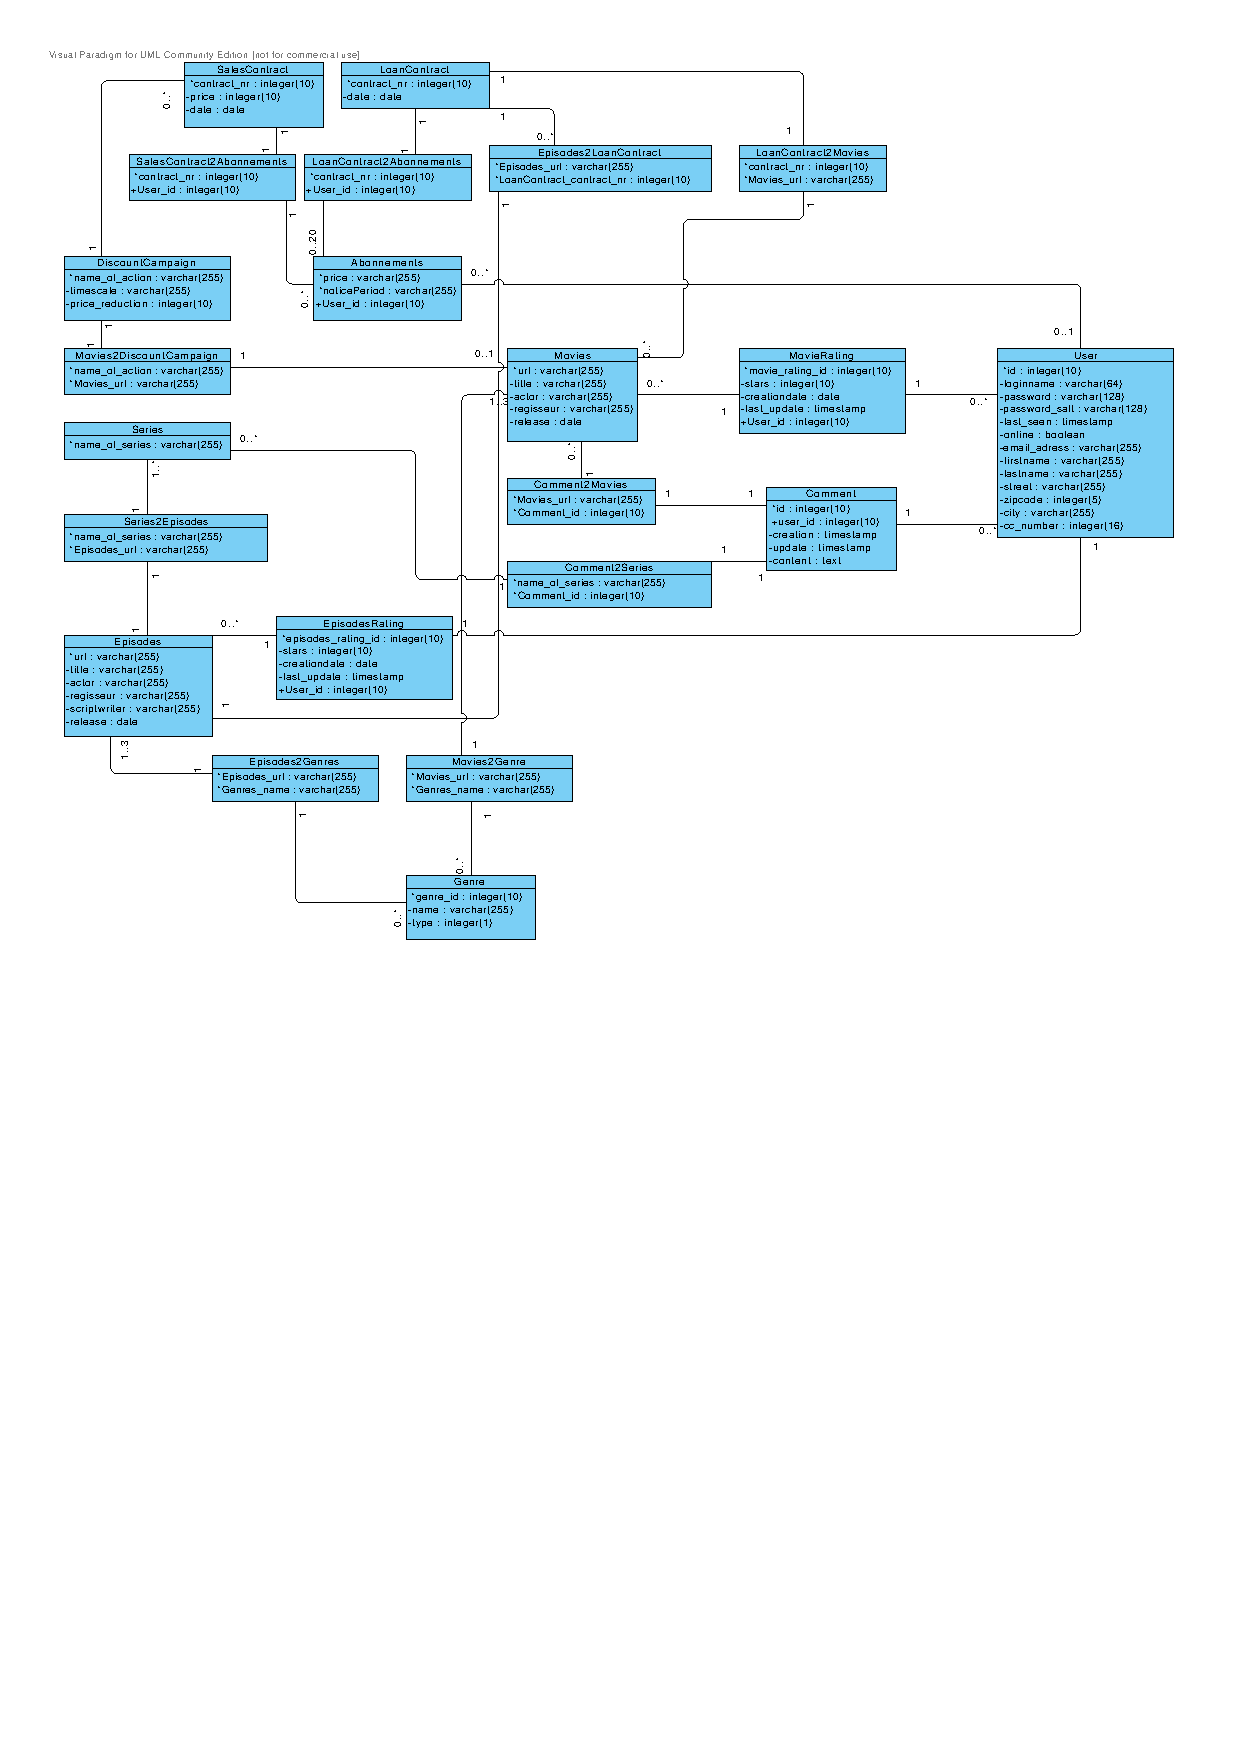
\includegraphics[page=1, angle=90,trim=0cm 0cm 1.1cm 1cm, clip=true, scale=1.1]{Diagramme/Paket_Netflax}
\end{document}